\makeatletter
\def\input@path{{../styles/}{../../styles/}{../../../styles/}{../}{../../}{../../../}}
\makeatother
\documentclass{ee102_notes}
% macros.tex - Course meta information
\renewcommand{\course}{EE 102}
\renewcommand{\coursetitle}{Signal Processing and Linear Systems}
\renewcommand{\instructor}{Ayush Pandey}
\renewcommand{\semester}{Fall}
\renewcommand{\year}{2025}
\renewcommand{\shorttitle}{Week 1: Introduction to Signals}
% Use \renewcommand to avoid 'already defined' errors

% The following packages can be found on http:\\www.ctan.org
% \usepackage{graphics} % for pdf, bitmapped graphics files
%\usepackage{epsfig} % for postscript graphics files
%\usepackage{mathptmx} % assumes new font selection scheme installed
%\usepackage{times} % assumes new font selection scheme installed
\usepackage{amsmath} % assumes amsmath package installed
\usepackage{amssymb,mathtools}  % assumes amsmath package installed
\usepackage{xcolor}
\usepackage{pgfplots,subcaption}
\usepackage[hidelinks]{hyperref}
\usepackage{verbatim}
\usepackage{graphicx}
\usepackage{listings}

% -------- listings (Python) ----------
\lstdefinestyle{py}{
  language=Python,
  basicstyle=\ttfamily\small,
  keywordstyle=\color{blue!60!black}\bfseries,
  commentstyle=\color{green!40!black},
  stringstyle=\color{orange!60!black},
  showstringspaces=false,
  columns=fullflexible,
  frame=single,
  framerule=0.3pt,
  numbers=left,
  numberstyle=\tiny,
  xleftmargin=1em,
  tabsize=2,
  breaklines=true,
}
\usepackage[american]{circuitikz}
\usepackage{tikz}
\usepackage{caption}    
\usepackage{lscape}
\usepackage{soul}
\usepackage{tikz}
\usetikzlibrary{calc,angles,quotes,arrows.meta}

\usepackage{hyperref}
\hypersetup{
    colorlinks=true,
    linkcolor=blue,
    filecolor=magenta,      
    urlcolor=blue,
    pdftitle={week1_notes},
    pdfpagemode=FullScreen,
}
%\usepackage{float} 

%\usepackage[demo]{graphicx}
\pgfplotsset{compat=1.18}
% \usepgfplotslibrary{fillbetween}

\newsavebox{\measurebox}

\let\proof\relax\let\endproof\relax


\newcommand{\norm}[1]{\left\lVert#1\right\rVert}
\def\abs#1{\left\lvert#1\right\rvert}
\let\proof\relax
\let\endproof\relax
\usepackage{amsthm}
\usepackage{accents}
\usepackage{relsize}
\newcommand{\ubar}[1]{\underaccent{\bar}{#1}}
\newtheorem{theorem}{Theorem}
\newtheorem{corollary}{Corollary}[theorem]
\newtheorem{lemma}{Lemma}
\newtheorem{proposition}{Proposition}
\newtheorem{statement}{Statement}

\theoremstyle{definition}
\newtheorem{definition}{Definition}
 
\theoremstyle{remark}
\newtheorem*{remark}{Remark}
\theoremstyle{remark}
\newtheorem*{claim}{Claim}
\setlength{\parindent}{0cm}
\newenvironment{nalign}{
    \begin{equation}
    \begin{aligned}
}{
    \end{aligned}
    \end{equation}
    \ignorespacesafterend
}

\renewcommand{\releasedate}{November 5, 2025}
\newcommand{\Eblank}{\rule{3cm}{0.4pt}}
\newcommand{\Rankblank}{\rule{3cm}{0.4pt}}

\begin{document}
\section*{EE 102 Week 10, Lecture 2 (Fall 2025)}
\subsection*{Instructor: \instructor}
\subsection*{Date: \releasedate}
\section{Announcements}
\begin{itemize}
    \item EE 122 Lab 02L is open and registration spots are available.
    \item HW \#9 is due on Mon Nov 10.
\end{itemize}
\section{Goals}
By the end of this lecture, you will be able to understand the Fourier Transform of discrete-time signals.

\section{Review: Fourier Transform in Continuous-Time}
The Fourier Transform (FT) of a continuous-time signal \( x(t) \) is defined as:
\[
X(\omega) = \int_{-\infty}^{\infty} x(t) e^{-j \omega t} dt
\]
where \( \omega \) is the angular frequency in radians per second. The Fourier transform provides a frequency-domain representation of the signal, allowing us to analyze its frequency components. That is, the signal, originally visualized with time as the X-axis, is now possible to be visualized with frequency ($\omega$) as the X-axis.

On the other hand, if you know how the signal behaves in the frequency domain, you can recover the time-domain signal using the Inverse Fourier Transform (IFT):
\[
x(t) = \frac{1}{2\pi} \int_{-\infty}^{\infty} X(\omega) e^{j \omega t} d\omega
\]
\section{Fourier Transform of Discrete-Time Signals}
For discrete-time signals, the Fourier Transform is defined similarly. What will you change in the two equations above? First, the variable \( t \) is replaced by \( n \), which represents discrete time indices (integers). That is, $n \in \mathbb{Z}$ while $t \in \mathbb{R}$ (all real numbers). Second, the integral will be replaced by a summation since we are dealing with discrete values (integration works for continuous values). Therefore, the Fourier Transform of a discrete-time signal \( x[n] \) is given by:
\begin{equation}
    \label{eq:dtft_intermediate}
    X(\dots) = \sum_{n=-\infty}^{\infty} x[n] e^{-j \omega n}
\end{equation}
Why the ``$\dots$'' in the equation above? 
\begin{popquiz}
    Is the Fourier Transform of a discrete-time signal a function of continuous frequency $\omega$ or discrete frequency $k$?
    \popqsplit 
    It is a continuous function of frequency $\omega$ (in radians) because $n$ gets summed over and $e^{-j \omega n}$ is defined for all real values of $\omega$.
\end{popquiz}
Notice that in the equation~\eqref{eq:dtft_intermediate}, we still have $\omega$ in the equation ($\omega \in \mathbb{R}$). So, the Fourier Transform of a discrete-time signal is a continuous function of frequency $\omega$ (in radians). This transform is called the Discrete-Time Fourier Transform (DTFT). Additionally, there are two reasons for \textbf{not} denoting it as $X(\omega)$. First, not a significant issue, but not denoting it as $X(\omega)$ helps to avoid confusion with the Fourier Transform of continuous-time signals (which is denoted as $X(\omega)$). 
The second issue is more important. Work on the following pop-quiz to understand it.
\begin{popquiz}
    Prove the following:
    \begin{itemize}
        \item The continuous-time complex exponential signal $x(t) = e^{j \omega t}$ is periodic \emph{in time} with period $T = \frac{2\pi}{\omega}$.
        \item The discrete-time complex exponential signal $x[n] = e^{j \omega n}$ is \textbf{periodic \emph{in frequency}} with period $2\pi$.
    \end{itemize}
    \popqsplit 
    For the continuous-time complex exponential signal, we apply the continuous time periodicity condition that must hold true for all periodic signals:
    \[
    x(t) = x(t + T)
    \]
    Substituting \( x(t) = e^{j \omega t} \) into the periodicity condition, we have:
    \[
    e^{j \omega t} = e^{j \omega (t + T)}
    \]
    Simplifying the right-hand side, we get:
    \[
    e^{j \omega t} = e^{j \omega t} e^{j \omega T}
    \]
    The term $e^{j \omega T}$ must equal 1 for the equality to hold for all \( t \). This leads to the condition:
    \[
    e^{j \omega T} = 1
    \]
    This occurs when $T = \frac{2\pi k}{\omega}$ for any integer \( k \). The fundamental period corresponds to \( k = 1 \), giving us:
    \[
    T = \frac{2\pi}{\omega}
    \]
    For the discrete-time complex exponential signal, we need to check periodicity in frequency. So, the condition that we need to check is:
    \[
      e^{j \omega n} = e^{j (\omega + \Omega) n}
    \]
    for some period \( \Omega \). We must find out what \( \Omega \) is. Simplifying the right-hand side, we have:
    \[
      e^{j \omega n} = e^{j \omega n} e^{j \Omega n}
    \]
    The term $e^{j \Omega n}$ must equal 1 for the equality to hold. This leads to the condition that $\Omega = 2 \pi k$ for any integer \( k \). The fundamental period corresponds to \( k = 1 \), giving us:
    \[
      \Omega = 2\pi
    \]
\end{popquiz}

The discrete-time complex exponential signal \( x[n] = e^{j \omega n} \) is periodic in frequency with period \( 2\pi \). This may be counter-intuitive -- why don't we have such a property in continuous-time? The key change from continuous-time to discrete-time is that time is now discrete (i.e., $n$ takes only integer values, rather than taking all values in $\mathbb{R}$). So, after every $2\pi$ increase in frequency, the discrete time complex exponential signal repeats itself because $n$ is an integer and any integer multiple of $2\pi$ in the exponent results in a full rotation around the unit circle. To see this more concretely, you can use Euler's identity to express the discrete-time complex exponential signal as:
\[
x[n] = e^{j \omega n} = \cos(\omega n) + j \sin(\omega n)
\]
After a $2\pi$ increase in frequency, we have:
\[
x[n] = e^{j (\omega + 2\pi) n} = e^{j \omega n} e^{j 2\pi n} = e^{j \omega n} (\cos(2\pi n) + j \sin(2\pi n)) = e^{j \omega n} (1 + j \cdot 0) = e^{j \omega n}
\]
So, you see the periodicity! If we follow through the same analysis in continuous-time, we will see that the periodicity does not hold for frequency. Given $x(t) = e^{j \omega t}$, after a $2\pi$ increase in frequency, we have:
\[
x(t) = e^{j (\omega + 2\pi) t} = e^{j \omega t} e^{j 2\pi t} = e^{j \omega t} (\cos(2\pi t) + j \sin(2\pi t))
\]
The term $\cos(2\pi t) + j \sin(2\pi t)$ does not equal 1 for all real values of \( t \), so the periodicity does not hold in continuous-time.

FINALLY, we can replace the ``$\dots$'' in equation~\eqref{eq:dtft_intermediate}. We have established two properties of the DTFT: it is a continuous function of frequency and it is periodic with period \( 2\pi \). Due to these two properties, we dentoe the DTFT as \( X(e^{j \omega}) \) to emphasize that it is a function of continuous frequency \( \omega \) and is periodic with period \( 2\pi \). Therefore, the final expression for the Discrete-Time Fourier Transform (DTFT) of a discrete-time signal \( x[n] \) is:
\begin{equation}
    \label{eq:dtft_final}
    X(e^{j \omega}) = \sum_{n=-\infty}^{\infty} x[n] e^{-j \omega n}
\end{equation}
Since the DTFT is a continuous function of frequency, the inverse DTFT will not involve summation over frequency (continuous variables are integrated). Therefore, the Inverse Discrete-Time Fourier Transform (IDTFT) is given by:
\begin{equation}
    \label{eq:idtft}
    x[n] = \frac{1}{2\pi} \int_{2\pi} X(e^{j \omega}) e^{j \omega n} d\omega
\end{equation}
The integration limit indicates that the integration is performed over one period of the DTFT, which is from \( 0 \) to \( 2\pi \) (or any other interval of length \( 2\pi \)) since the DTFT is periodic with period \( 2\pi \).

\section{Properties of DTFT}
\subsection{Periodicity}
We have discussed how the discrete-time complex exponential signal is periodic in frequency with period \( 2\pi \). Using that, we can show that the DTFT is also periodic with period \( 2\pi \). To see this, consider the DTFT expression in equation~\eqref{eq:dtft_final}:
\[
X(e^{j (\omega + 2\pi)}) = \sum_{n=-\infty}^{\infty} x[n] e^{-j (\omega + 2\pi) n} = \sum_{n=-\infty}^{\infty} x[n] e^{-j \omega n} e^{-j 2\pi n} = X(e^{j \omega})
\] 
Thus, the DTFT is periodic with period \( 2\pi \).
\subsection{Linearity}
Just like the continuous-time Fourier Transform, the DTFT is also linear. That is, if you have two discrete-time signals \( x_1[n] \) and \( x_2[n] \) with DTFTs \( X_1(e^{j \omega}) \) and \( X_2(e^{j \omega}) \) respectively, then for any constants \( a \) and \( b \), the DTFT of the linear combination \( y[n] = a x_1[n] + b x_2[n] \) is given by:
\[Y(e^{j \omega}) = a X_1(e^{j \omega}) + b X_2(e^{j \omega})\]
\subsection{Time Shifting}
If a discrete-time signal \( x[n] \) has a DTFT \( X(e^{j \omega}) \), then the DTFT of the time-shifted signal \( x[n - n_0] \) is given by:
\[X_{\text{shifted}}(e^{j \omega}) = X(e^{j \omega}) e^{-j \omega n_0}\]
This property indicates that a shift in the time domain corresponds to a multiplication by a complex exponential in the frequency domain.
\subsection{Frequency Shifting}
If a discrete-time signal \( x[n] \) has a DTFT \( X(e^{j \omega}) \), then the DTFT of the frequency-shifted signal, with shifted frequency: $\omega_{\text{shifted}} = \omega - \omega_0$, is given by $X(e^{j (\omega - \omega_0)})$. This can be written as 
\[ X(e^{j(\omega - \omega_0)}) = X(e^{j \omega}) e^{j \omega_0 n}\]
\subsection{Convolution}
The convolution property, as discussed in the previous lecture, is among the most important property for signal processing applications. For a system with impulse response \( h[n] \) and input signal \( x[n] \), the output signal \( y[n] \) is given by the convolution of \( x[n] \) and \( h[n] \):
\[y[n] = x[n] * h[n] = \sum_{k=-\infty}^{\infty} x[k] h[n - k]\]
The DTFT of the output signal \( y[n] \) is given by the product of the DTFTs of the input signal and the impulse response:
\[Y(e^{j \omega}) = X(e^{j \omega}) H(e^{j \omega})\]
This is useful because now you get full control over the design of the system by designing the frequency response \( H(e^{j \omega}) \) to achieve the desired output characteristics.

\section{Examples: Filtering}
Let's start with a simple example. Consider the design of an audio processing system. So, our goal is to design $h(t)$ in time-domain (or if it is easier, we might design $H(j\omega)$ in frequency-domain) to achieve the desired output characteristics. Let's say that there is an audio input signal $x(t)$ and we only want to keep the three most dominant frequency components of the signal and remove all other frequency components in the output. If the three most dominant frequency components are at frequencies $\omega_1$, $\omega_2$, and $\omega_3$, then we can design the frequency response of the system as follows:
\[
H(j\omega) = \begin{cases}
    1, & \text{if } \omega \in (\omega_1 - \Delta \omega, \omega_1 + \Delta \omega) \\
    1, & \text{if } \omega \in (\omega_2 - \Delta \omega, \omega_2 + \Delta \omega) \\
    1, & \text{if } \omega \in (\omega_3 - \Delta \omega, \omega_3 + \Delta \omega) \\
    0, & \text{otherwise}
\end{cases}
\]
where \( \Delta \omega \) is a small frequency range around each dominant frequency component. This design allows only the desired frequency components to pass through while attenuating all other frequencies (because of the convolution property). 
\subsection{Filtering an audio mix}
Consider an audio signal where you have three frequency tones mixed together:
\[
x(t) = \cos(t) + \cos(5t) + \cos(100t)
\]
The three frequency components are at \( \omega_1 = 1 \) rad/s, \( \omega_2 = 5 \) rad/s, and \( \omega_3 = 100 \) rad/s. Our goal is to design a filter that only allows the frequency component at \( \omega_2 = 5 \) rad/s to pass through while attenuating the other two frequency components. We can achieve this by designing the frequency response of the audio processing system. Then, by using the convolution property, the output Fourier Transform will be the product of the input Fourier Transform and the designed frequency response. Finally, we can use the Inverse Fourier Transform to recover the time-domain output signal.

The first step is to compute the Fourier Transform of the input signal \( x(t) \). 
\begin{popquiz}
    What is the Fourier Transform of \( x(t) = \cos(\omega_0 t) \)? Start by predicting what you expect the $\cos(t)$ signal to look like in the frequency domain? Hint: It's just one frequency component. 
    % draw a cos(t) on left in time-domain and draw a delta at omega=1 and omega=-1 on right in frequency-domain with $\omega$ as x-axis on the right.
    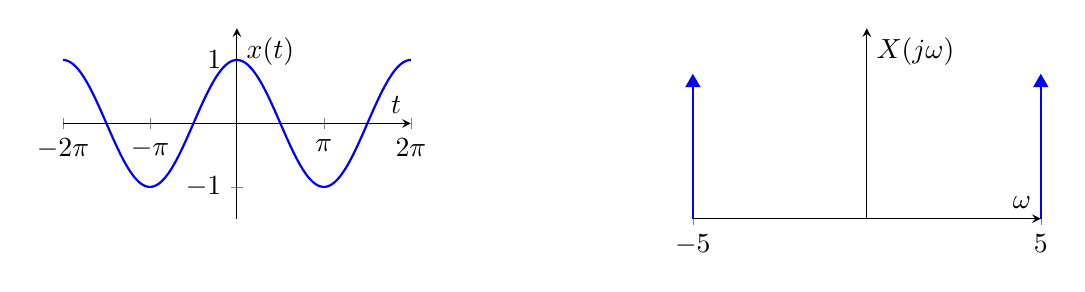
\begin{tikzpicture}
  %----- time-domain axis -----
  \begin{axis}[
    axis lines=middle,
    xlabel={$t$},
    ylabel={$x(t)$},
    xtick={-6.2832,-3.1416,0,3.1416,6.2832},
    xticklabels={$-2\pi$,$-\pi$,$0$,$\pi$,$2\pi$},
    ytick={-1,0,1},
    ymin=-1.5, ymax=1.5,
    width=6cm,
    height=4cm,
    domain=-6.2832:6.2832,
    samples=200
  ]
    \addplot[blue, thick] {cos(deg(x))};
  \end{axis}

  %----- frequency-domain axis (impulses) -----
  \begin{axis}[
    axis lines=middle,
    xlabel={$\omega$},
    ylabel={$X(j\omega)$},
    xtick={-5,0,5},
    xticklabels={$-5$,$0$,$5$},
    ytick=\empty,
    ymin=0, ymax=1.4,
    width=6cm,
    height=4cm,
    xshift=8cm,
    clip=false
  ]
    % vertical impulse "stems" with arrowheads
    \addplot+[
      ycomb,
      blue,
      thick,
      mark=triangle*,
      mark options={scale=1.2},
    ] coordinates {(-5,1) (5,1)};
    % optional labels for amplitudes (e.g., \pi)
    %\node[above, blue] at (axis cs:-5,1) {$\pi$};
    %\node[above, blue] at (axis cs:5,1) {$\pi$};
  \end{axis}
\end{tikzpicture}

    \popqsplit 
    Intuitively, we expect the Fourier Transform of \( \cos(\omega_0 t) \) to consist of impulse at the frequency components \( \omega = \omega_0 \). However, because we work with complex exponentials, we actually have two impulses: one at \( \omega = \omega_0 \) and another at \( \omega = -\omega_0 \). The negative frequency arises due to the Euler's formula representation of cosine (which converts the complex to the real):
    \[
    \cos(\omega_0 t) = \frac{1}{2} \left( e^{j \omega_0 t} + e^{-j \omega_0 t} \right)
    \]
    So, it's clear that there is a frequency at $\omega_0$ and another frequency at $-\omega_0$.
\end{popquiz}
To see the Fourier transform of a cosine signal formally, compute the inverse Fourier Transform of the following signal:
\[ 
X(\omega) = 2 \pi \delta(\omega - \omega_0)
\]

The inverse Fourier Transform is given by:
\[
x(t) = \frac{1}{2\pi} \int_{-\infty}^{\infty} X(\omega) e^{j \omega t} d\omega
\]
(you can see the reason why we have $2\pi$ in front of the delta function --- so it cancels out with the $\frac{1}{2\pi}$ term in front of the integral in the inverse Fourier Transform equation).

Substituting \( X(\omega) = 2 \pi \delta(\omega - \omega_0) \) into the inverse Fourier Transform equation, we have:
\[
x(t) = \frac{1}{2\pi} \int_{-\infty}^{\infty} 2 \pi \delta(\omega - \omega_0) e^{j \omega t} d\omega
\]
now, using the sifting property of the delta function, we can evaluate the integral:
\[
x(t) = e^{j \omega_0 t}
\]
since the area under curve of the impulse is $1$, we get $e^{j \omega_0 t}$.

So, we have the Fourier Transform pair:
\[
X(\omega) = 2 \pi \delta(\omega - \omega_0) \quad \leftrightarrow \quad x(t) = e^{j \omega_0 t}
\]
Now, using Euler's formula, we can express the cosine function in terms of complex exponentials:
\[
\cos(\omega_0 t) = \frac{1}{2} \left( e^{j \omega_0 t} + e^{-j \omega_0 t} \right)
\]
So, the Fourier Transform of \( \cos(\omega_0 t) \) can be derived by taking the Fourier Transform of each exponential term separately and adding them together by using the linearity property of the Fourier Transform.

\[
\mathcal{F}\{ \cos(\omega_0 t) \} = \frac{1}{2} \left( \mathcal{F}\{ e^{j \omega_0 t} \} + \mathcal{F}\{ e^{-j \omega_0 t} \} \right)
\]

We get, 
\[
\mathcal{F}\{ \cos(\omega_0 t) \} = \frac{1}{2} \left( 2 \pi \delta(\omega - \omega_0) + 2 \pi \delta(\omega + \omega_0) \right) 
= \pi \left( \delta(\omega - \omega_0) + \delta(\omega + \omega_0) \right)
\]

So, now we can write $X(\omega)$ for our input signal \( x(t) = \cos(t) + \cos(5t) + \cos(100t) \):
\[
X(\omega) = \pi \left( \delta(\omega - 1) + \delta(\omega + 1) \right) + \pi \left( \delta(\omega - 5) + \delta(\omega + 5) \right) + \pi \left( \delta(\omega - 100) + \delta(\omega + 100) \right)
\]
Our goal is to design a filter that only allows the frequency component at \( \omega = 5 \) rad/s to pass through while attenuating the other two frequency components. Therefore, we can design the frequency response of the audio processing system as follows:
\[
H(j\omega) = \begin{cases}
    1, & \text{if } \omega \in (5 - \Delta \omega, 5 + \Delta \omega) \\
    0, & \text{otherwise}
\end{cases}
\]
where \( \Delta \omega \) is a small frequency range around \( 5 \) rad/s. Visually, this frequency response is shown in Figure~\ref{fig:frequency_response_example}.
\begin{figure}[h]
    \centering
    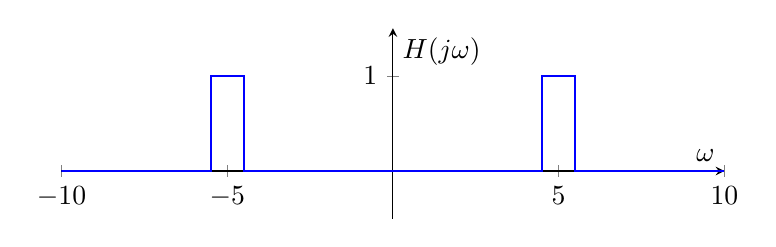
\begin{tikzpicture}
  \begin{axis}[
    axis lines=middle,
    xlabel={$\omega$},
    ylabel={$H(j\omega)$},
    xmin=-10, xmax=10,
    ymin=-0.5, ymax=1.5,
    xtick={-10,-5,0,5,10},
    xticklabels={$-10$,$-5$,$0$,$5$,$10$},
    ytick={0,1},
    width=10cm,
    height=4cm
  ]
    % Ideal two-line passband around ±5 (here width = 1: [4.5,5.5] and [-5.5,-4.5])
    \addplot[blue, thick] coordinates {
      (-10,0) (-5.5,0) (-5.5,1) (-4.5,1) (-4.5,0)
      ( 4.5,0) ( 4.5,1) ( 5.5,1) ( 5.5,0) (10,0)
    };
  \end{axis}
\end{tikzpicture}

    \caption{Frequency response of the designed filter.}
    \label{fig:frequency_response_example}
\end{figure}
The output Fourier Transform \( Y(\omega) \) is given by the product of the input Fourier Transform \( X(\omega) \) and the designed frequency response \( H(j\omega) \):
\[
Y(\omega) = X(\omega) H(j\omega)
= \pi \left( \delta(\omega - 5) + \delta(\omega + 5) \right)
\]
because all other impulses are multiplied by zero.

Finally, we can use the Inverse Fourier Transform to recover the time-domain output signal \( y(t) \):
\[
y(t) = \frac{1}{2\pi} \int_{-\infty}^{\infty} Y(\omega) e^{j \omega t} d\omega
= \frac{1}{2\pi} \int_{-\infty}^{\infty} \pi \left( \delta(\omega - 5) + \delta(\omega + 5) \right) e^{j \omega t} d\omega
\]
\[
= \frac{1}{2} \left( e^{j 5 t} + e^{-j 5 t} \right) = \cos(5t)
\]
Thus, the output signal \( y(t) \) contains only the frequency component at \( \omega = 5 \) rad/s, as desired.

\subsection{Discrete-time example: filtering}
Now let's consider a discrete-time example. Although it might seem that the story will proceed similarly, there are some important differences due to the periodicity of the DTFT! We have a discrete-time signal where three frequency tones are mixed together:
\[
x[n] = \cos(n) + \cos(5n) + \cos(100n)
\]
Let's assume that we want an ideal filter that removes the component at $100$ rad/s (after wrapping into $(-\pi,\pi]$) while keeping the components at $\omega=\pm 1$ and $\omega=\pm 5$.

Write the DTFT
\[
\mathcal{F}\{\cos(\omega_0 n)\} \;=\; \pi\big[\delta(\omega-\omega_0)+\delta(\omega+\omega_0)\big],
\]

The tones at $\omega=1$ and $\omega=5$ already lie in $(-\pi,\pi]$. The tone at $100$ must be wrapped into $(-\pi,\pi]$:
\[
100 - 32\pi \;\approx\; -0.53\ \text{rad}.
\]
Hence, over one principal period $(-\pi,\pi]$, the three tones appear at
\[
\omega=\pm 1,\qquad \omega=\pm 5,\qquad \omega=\pm 0.53.
\]
Therefore,
\[
X(e^{j\omega})
=\pi\sum_{\omega_0\in\{1,\,5,\,0.53\}}
\big[\delta(\omega-\omega_0)+\delta(\omega+\omega_0)\big]
\]
We want to keep $\omega=\pm 1,\pm 5$ and reject $\omega=\pm 0.53$. Even though the frequency we wanted to remove was 100 rad/s, after wrapping into $(-\pi,\pi]$, it became $-0.53$ rad/s --- so, if you thought that you could design a low-pass filter to remove high frequencies, you would be mistaken! In this case, we instead need a high-pass filter! 

So, let's design a high-pass filter with cutoff between $0.53$ and $1$; for instance,
\[
\omega_c=0.5
\]
Define
\[
H(e^{j\omega}) \;=\;
\begin{cases}
0, & |\omega|<\omega_c,\\[4pt]
1, & \omega_c\le |\omega|\le \pi,
\end{cases}
\qquad\text{extended $2\pi$-periodically.}
\]

Now, using the convolution property, the output DTFT is
\[
Y(e^{j\omega}) \;=\; H(e^{j\omega})\,X(e^{j\omega}).
\]
The impulses at $\omega=\pm 0.53$ lie in $(-\omega_c,\omega_c)$. So, these go away! While the impulses at $\omega=\pm 1,\pm 5$ are passed through. We have,
\[
Y(e^{j\omega})
=\pi\big[\delta(\omega-1)+\delta(\omega+1)+\delta(\omega-5)+\delta(\omega+5)\big].
\]
Taking the inverse DTFT by inspection,
\[
y[n] \;=\; \cos(n) \;+\; \cos(5n).
\]

Finally, we can derive the impulse response using the inverse Fourier transform (if needed).

\section{Computational implementation of the DTFT}
Although the previous example worked fine, there are some practical issues with implementing the DTFT on a computer. First, the DTFT integral in equation~\eqref{eq:dtft_final} is defined over an infinite range (from $-\infty$ to $\infty$). Computers only have finite computations! Second, the DTFT is a continuous function of frequency, but in practice, we can only compute it at discrete frequency points (everything in computers is finite). To address these issues, we sample the Discrete-Time Fourier Transform at specific frequencies. This leads to a new Fourier transform called the Discrete Fourier Transform (DFT). The DFT is defined for a finite-length discrete-time signal \( x[n] \) of length \( N \) as:
\begin{equation}
    \label{eq:dft}
X[k] = \sum_{n=0}^{N-1} x[n] e^{-j \frac{2\pi}{N} k n}, \quad k = 0, 1, 2, \ldots, N-1
\end{equation}
where \( k \) represents the discrete frequency index. The DFT provides a frequency-domain representation of the finite-length discrete-time signal, allowing us to analyze its frequency components at specific discrete frequencies.

\textbf{What changed?}
\begin{itemize}
    \item You have a time-domain signal of finite length \( N \) (from \( n = 0 \) to \( n = N-1 \)). This is your computational array that stores the signal. 
    \item You compute the Fourier Transform at discrete frequency points \( k = 0, 1, 2, \ldots, N-1 \), not in radians but in terms of indices. Notice how the total number of frequency points is also \( N \).
    \item The frequency resolution is determined by the length of the signal \( N \). Due to this, we are able to write $\omega$ as $\omega = \frac{2\pi}{N} k$ in the DFT equation, that is integer multiples of the fundamental frequency spacing \( \frac{2\pi}{N} \).
    \item The frequency spacing between adjacent DFT bins is given by \( \Delta f = \frac{1}{N} \) (in cycles per sample) or \( \Delta \omega = \frac{2\pi}{N} \) (in radians per sample).
\end{itemize}

From the DFT, you can recover the time-domain signal using the Inverse Discrete Fourier Transform (IDFT):
\begin{equation}
    \label{eq:idft}
x[n] = \frac{1}{N} \sum_{k=0}^{N-1} X[k] e^{j \frac{2\pi}{N} k n}, \quad n = 0, 1, 2, \ldots, N-1
\end{equation}
The IDFT allows you to reconstruct the original finite-length discrete-time signal from its DFT representation.

Equations~\eqref{eq:dft} and~\eqref{eq:idft} form the basis for many signal processing applications and these are the two computationally feasible equations you are expected to apply in Homework \#9.

\section{Recommended Reading}
Read the Wikipedia page on Discrete Fourier Transform (DFT) -- it can be confusing! But as a student in EE 102, you might now be one of those few people in the world who are able to \emph{understand} this difficult topic!
\end{document}